% Aus der Datei preambel.tex werden alle globalen Einstellungen für das Dokument geladen:
\documentclass[a4paper,11pt,ngerman,DIV=12,BCOR=12mm,titlepage,toc=listof,toc=bib]{scrartcl}

\usepackage{cmap} % to make the PDF files "searchable and copyable" in pdf viewer
\usepackage[T1]{fontenc}
\usepackage[utf8]{inputenc}
\usepackage[ngerman]{babel}
\usepackage[babel,german=quotes]{csquotes}
\usepackage{bibgerm}
\usepackage[authoryear]{natbib}
\usepackage[font=small,labelfont=bf,format=hang]{caption} % viele Formatierungsmöglichkeiten für die Bildunterschriften

\usepackage[scaled]{beramono} % Monospace Font im Dokument
\usepackage{libertine}
\renewcommand*\familydefault{\sfdefault}  %% Only if the base font of the document is to be sans serif

\usepackage{microtype}		% echter Blocksatz
\usepackage{fixltx2e}		% Verbessert einige Kernkompetenzen von LaTeX2e
\usepackage{ellipsis}		% Korrigiert den Weißraum um Auslassungspunkte
\usepackage{color}
\usepackage{graphicx}		% Paket zum Einbinden von Grafiken:
\usepackage{array}		%Paket für Tabellen
\usepackage[thinqspace, textstyle]{SIunits} %Syntax: \unit{0}{\kelvin} sind \unit{273}{\celsius} oder z.b. {\watt\per\square\meter}, oder \unit{12}{\kilo\square\meter} für Quadratkilometer

%\usepackage{amsmath} % Auskommentieren, wenn mathematische Formeln gesetzt werden sollen.

% Support for PDF inclusion
\usepackage[final]{pdfpages}

\usepackage{setspace}		% Paket für halben Zeilenabstand
%\doublespacing			% doppelter Zeilenabstand
\onehalfspacing			% Zeilenabstand 1,5

%%% Listings (Quelltext-Darstellungen) formatieren %%%
\usepackage{listings}
\definecolor{codegray}{gray}{.95}
\definecolor{darkblue}{rgb}{0,0,.6}
\definecolor{darkred}{rgb}{.6,0,0}
\definecolor{darkgreen}{rgb}{0,.6,0}
\definecolor{red}{rgb}{.98,0,0}
\definecolor{Tgreen}{HTML}{73D216}	% tango chameleon 2#
\definecolor{Tlilacdark}{HTML}{5C3566}	% tango plum 3
\definecolor{Tlilac}{HTML}{75507B}	% tango plum 2
\lstset{basicstyle=\footnotesize\ttfamily, frame=single, backgroundcolor=\color{white}, breaklines, 		showstringspaces=false,
  commentstyle=\color{Tlilac}, keywordstyle=\bfseries\color{Tgreen}, stringstyle=\color{darkred},
  xleftmargin=0.5cm, numbers=left, numberstyle=\footnotesize, stepnumber=1, numbersep=5pt, 
  literate={ö}{{\"o}}1 % Probleme mit Umlauten in Codeumgebungen umgehen
           {ä}{{\"a}}1
           {ü}{{\"u}}1
           {ß}{{ss}}1
}

\renewcommand*\lstlistlistingname{Script-Verzeichnis} % Umbenennen des Listing-Verz. in Script-Verz.
\renewcommand*\lstlistingname{Script} % Umbenennen des Listings in Script

%%% Hyperref-Paket
\usepackage[
	colorlinks,
	pdfpagelabels,
	pdfstartview = FitH,
	bookmarksopen = true,
	bookmarksnumbered = true,
	linkcolor = black,
	plainpages = false,
	hypertexnames = false,
	citecolor = black,
	urlcolor=black,
	pdftitle={Titel der Arbeit}, %%% Titel eintragen, erscheint automatisch in den PDF Eigenschaften
	pdfauthor={Autor der Arbeit} %%% Autor eintragen, erscheint automatisch in den PDF Eigenschaften
]{hyperref}

%%% Seitenlayout mit dem KOMA-Paket
\usepackage[%
   % headtopline,
   % plainheadtopline,
    headsepline,
   % plainheadsepline,
    footsepline,
   % plainfootsepline,
   % footbotline,
   % plainfootbotline,
   % ilines,
   % clines,
   % olines,
   automark,
   % autooneside,% ignore optional argument in automark at oneside
   komastyle,
%    standardstyle,
   % markuppercase,
   % markusedcase,
%   nouppercase,
]{scrpage2}


%%%%%%%%%%%%%%%%%%%%%%%%%%%%%%%%%%%%%%%%%%%%%%%%%%%%%
% Schusterjungen und Hurenkinder vermeiden
\clubpenalty = 10000
\widowpenalty = 10000
\displaywidowpenalty = 10000



%%% Hier wird die Titelseite angepasst:

% Seitenrahmen und Nummerierungen ausschalten
\pagestyle{empty}

% fuer den Anfang roemische Seitennummern
\pagenumbering{Roman}    % roman | arabic


\titlehead{Freie Universität Berlin\\
           Fachbereich Geowissenschaften\\
           Institut für Geographische Wissenschaften}

\subject{Hausarbeit}

\title{Titel der Hausarbeit}

%\subtitle{Untertitel, wenn benötigt} 

% Name des oder der Autoren eintragen
\author{Autor 1, Autor 2, Autor 3}

% Datum wird automatisch eingetragen beim kompilieren, für manuell einfach ersetzen!
\date{\today} 

% Anpassen nach Bedarf, für einzeilig einfach die \\ wegnehmen
\publishers{Dozenten:\\Prof. Dr. Dozent 1\\Prof. Dr. Dozent 2}


%%% Beginn des eigentlichen Dokuments

%%%%%%%%%%%%%%%%%%%%%%%%%%%%%%%%%%%%%%%%%%%%%%%%%%
\begin{document}
%%%%%%%%%%%%%%%%%%%%%%%%%%%%%%%%%%%%%%%%%%%%%%%%%%

\maketitle % Titelseite hier jetzt erstellen
\clearpage


\pagestyle{scrheadings}    % wieder auf normale Seitenrahmen zurück schalten
\clearscrheadfoot

\automark[subsection]{section}
\cfoot{\pagemark}
\chead{\headmark}

% Inhaltsverzeichnis in den PDF-Links eintragen
\pdfbookmark[1]{Inhaltsverzeichnis}{toc}

%%% Inhaltsverzeichnis 
\tableofcontents

\newpage

%%% Abbildungsverzeichnis 
\listoffigures

%%% Tabellenverzeichnis 
\listoftables

%%% Listings-Verzeichnis 
\lstlistoflistings


%%%%%%%%%%%%%%%%%%%%%%%%%%%%%%%%%%%%%%%%%%%%
\newpage % Beginn des Textkörpers
%%%%%%%%%%%%%%%%%%%%%%%%%%%%%%%%%%%%%%%%%%%%

%% Für den Hauptteil normale Seitenzahlen
\pagenumbering{arabic}  % Nummerierungstyp roman | arabic

\section{Einleitung}
\subsection{Unterkapitel 1}

%Beispiele
Wie \cite{nachname_2005} berichtet, siehe auch Abbildung \ref{fig:Beispiel.png}, Lorem ipsum dolor sit amet, consetetur sadipscing elitr, sed diam nonumy eirmod tempor invidunt ut labore et dolore magna aliquyam erat, sed diam voluptua. At vero eos et accusam et justo duo dolores et ea rebum. Stet clita kasd gubergren, no sea takimata sanctus est Lorem ipsum dolor sit amet. Lorem ipsum dolor sit amet, consetetur sadipscing elitr, sed diam nonumy eirmod tempor invidunt ut labore et dolore magna aliquyam erat, sed diam voluptua. At vero eos et accusam et justo duo dolores et ea rebum. Stet clita kasd gubergren, no sea takimata sanctus est Lorem ipsum dolor sit amet. Lorem ipsum dolor sit amet, consetetur sadipscing elitr, sed diam nonumy eirmod tempor invidunt ut labore et dolore magna aliquyam erat, sed diam voluptua. At vero eos et accusam et justo duo dolores et ea rebum. Stet clita kasd gubergren, no sea takimata sanctus est Lorem ipsum dolor sit amet \citep[vgl.][gemäß freundlicher persönlicher Mitteilung]{nachname_2005}.

\begin{figure}[htb] % Wo das Bild gesetzt wird, entscheidet LaTeX nach Typographischen Aspekten. Wenn ein Bild gesetzt werden soll, bevor ein neues Kapitel anfängt, muss nach dem alten Kapitel der Befehl \clearpage eingesetzt werden. Dann werden alle Float-Umgebungen, die noch "in der Luft hängen", gesetzt.
\centering
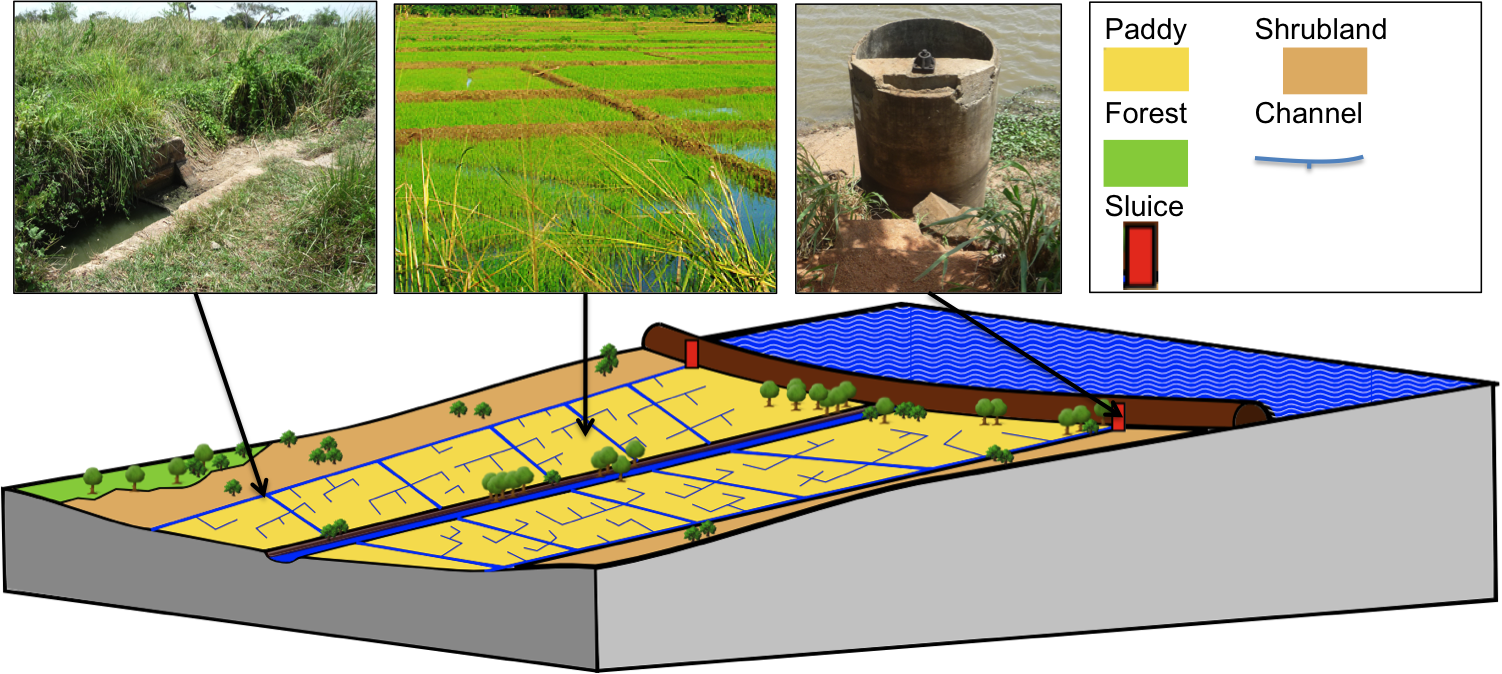
\includegraphics[width=0.8\textwidth]{images/Beispiel.png} % 0.8/textwidth setzt das Bild in 0,8-facher Textbreite. Der Faktor kann variiert oder weggelassen werden. Es gibt auch \textheight! Beachte bei Karten mit Maßstab, dass dieser beim Skalieren verändert wird!
\caption[Bildunterschrift für das Abb.Verz.]{Bildunterschrift \citep[aus:][]{nachname_2005}}
\label{fig:Beispiel.png} % Gibt man im Text \ref{fig:Beispiel.png} an, wir dort automatisch die Nummer des Bildes gesetzt.
\end{figure}



\subsection{Unterkapitel 2}

Lorem ipsum dolor sit amet, consetetur sadipscing elitr, sed diam nonumy eirmod tempor invidunt ut labore et dolore magna aliquyam erat, sed diam voluptua. At vero eos et accusam et justo duo dolores et ea rebum. Stet clita kasd gubergren, no sea takimata sanctus est Lorem ipsum dolor sit amet. Lorem ipsum dolor sit amet, consetetur sadipscing elitr, sed diam nonumy eirmod tempor invidunt ut labore et dolore magna aliquyam erat, sed diam voluptua. At vero eos et accusam et justo duo dolores et ea rebum. Stet clita kasd gubergren, no sea takimata sanctus est Lorem ipsum dolor sit amet. Lorem ipsum dolor sit amet, consetetur sadipscing elitr, sed diam nonumy eirmod tempor invidunt ut labore et dolore magna aliquyam erat, sed diam voluptua. At vero eos et accusam et justo duo dolores et ea rebum. Stet clita kasd gubergren, no sea takimata sanctus est Lorem ipsum dolor sit amet.   

\subsubsection{Unterunterkapitel}


\clearpage

\section{Untersuchungsgebiet}
\input{content/2_Untersuchungsgebiet.tex}

\clearpage

\section{Methoden}
\input{content/3_Methoden.tex}

\clearpage

\section{Ergebnisse}
\input{content/4_Ergebnisse.tex}

\clearpage

\section{Diskussion}
\input{content/5_Diskussion.tex}

\clearpage

\section{Zusammenfassung}
\input{content/6_Fazit.tex}

\clearpage

%%%%%%%%%%%%%%%%%%%%%%%%%%%%%%%%%%%%%%%%%%%%%%%%
% Ende des Textkörpers
%%%%%%%%%%%%%%%%%%%%%%%%%%%%%%%%%%%%%%%%%%%%%%%%


%%% Literatur-Verzeichnis 

% damit wird die Datei literature.bib aus dem gleichen Verzeichnis benutzt. Zum Bearbeiten der Datei empfehle ich pybliographer oder Zotero!
\bibliography{literature} 

% hier einen passenden Stil für die Darstellung der Zitate im Text und im Lit.-Verz. angeben!
\bibliographystyle{munich} 

\newpage

%%% Anhang %%%%%%%%%%%%%%%%%%%%%%%%%%%%%%%%%%%%%

\pagestyle{plain} 

\section*{Anhang} % Kapitel ohne Nummerierung
\addcontentsline{toc}{section}{Anhang}

\begin{appendix}

% Hier können jetzt nach belieben Bilder, Tabellen, Karten und sogar ganze PDF-Dokumente eingebunden werden! Z.B.:


%\begin{figure}[htb]
%\centering
%\includegraphics[width=\textwidth]{images/map.png}
%\caption{Bildunterschrift}
%\label{fig:map.png}
%\end{figure}


% EInbindung PDF Seiten according to : http://gb01.blogspot.de/2008/03/include-pdf-in-latex.html
% Globals: include all pages, don't auto scale
%\includepdfset{pages=-}

% Include the PDF files, scaling as required
%% \includepdf[scale=1.25]{title.pdf}
%\includepdf[landscape, fitpaper]{images/map.pdf}



\end{appendix}
%%%%%%%%%%%%%%%%%%%%%%%%%%%%%%%%%%%%%%%%%%%%%%%%%
\end{document}
